\chapter{动态规划}\label{Sec:Chapter:DynamicProgramming}
\section{概述}
\noindent\emph{Those who cannot remember the past are condemned to repeat it.}\\
\indent \indent \emph{-George Santayana, The Life of Reason; or,}\\
\indent \indent \emph{The Phases of Human Progress(1905)}

在计算机科学中动态规划已经演化成一种主要的算法设计范例。但是它的名字对于
许多人有点神秘。这个名字是1957年由Richard Bellman在描述一种最优控制问题
时构造的。实际上,名字来源与描述的问题而不是解决问题的技术。这里programming
表示“一系列选择”,比如规划一个无线电站。词动态的(dynamic)表示一种思想,
即选择依赖于当前的状态,而不是在之前就决定好了。所以在原来意思里面,a
radio show in which listeners call in request might might be said to
be "dynamically programmed" to contrast it with the more usual
format where the selections are decided before the show begins.
Bellman描述了一种解决“dynamically  programming”问题的方法,这种方法成
了后来好多计算机算法的灵感。这个方法的主要特点是将指数时间的问题转换成
多项式时间。这称为了动态规发算法的主要特点。

本章不同与其他章,其他章中我们经常关注某个问题或应用领域并各方法来解决之;
但是在本章中,我们关注一种技术,为不同应用领域开发动态规划解决方案的技术。

自顶向下的算设计是自然的且强大的。我们首先在通用方式上考虑和计划,之后在
增加细节。我们通过将顶层复杂的问题分解成子问题来解决之。使用递归,我们通过
将大型问题分解成同样的小规模问题来解决。分而治之,这种递归算法设计技术,被
证明在得到快速的排序算法时是很有用的。但是象好的递归一样,如果不正确的控制,
它仍然将变的非常低效。Fibonacci数列提供了一个简单而深刻的例子。

\begin{example}
递归的Fibonacci函数

回忆等式\ref{Equa:FibonacciSeries},Fibonacci数列以递归等式定义
$F_n=F_{n-1}+F_{n-2}$对于$n\geq 2$,边界值是$F_0=0,F_1=1$。他们是递归定义的,
所以自然而然的计算他们就使用例3.1给出的递归函数fib(n)。但是,如图7.13所示,
自然的递归计算有可怕的低效率,因为进行了大量的重复工作。图7.13实质上展示了
fib(6)的活动记录树。一般的,fib(n)的活动记录树是一颗深度为n/2(最右边的路径最短)
的完全二叉树,而且在更低的深度有更多的节点,所以运行时间至少是$\Omega(2^{n/2})$。
练习10.1会给出一个精确的渐进阶。但是$F_n$可以由$\Theta(n)$简单语句的算法计算出,
只需要计算并记录比n小的值就可以了,如果小的值都是已知的话计算fib(n)只需要
常量时间。(复习3.2.1小节,简单语句就是不调用函数,需要常量时间执行的语句。)
假设有一个大数组f,下面的代码:
\begin{lstlisting}[language={Java},keywordstyle=\color{blue!70}, commentstyle=\color{red!50!green!50!blue!50}]
f[0]=0; f[1]=1
for(i=2; i<=n; i++)
    f[u]=f[i-1]+f[i-2];
\end{lstlisting}
练习10.2dispenses with the 数组。
\end{example}

一个动态规划算法为子问题存储结果或是解决方案,之后在需要他们来解决大型问题的
时候,就可以直接查找他们而不是重新计算。因此动态规划特别适合那些递归算法会
重复解决很多子问题的问题。

We will introduce a characterization of dynamic programming algorithms that
provides a unified framework for a wide variety of published algorithms that
might seem quite different on the surface. 这套framework允许将一个递归解决
方案转换成一个动态规划算法,提供了分析动态规划算法复杂度的方法。

\section{子问题图和他们的的遍历}\label{Sec:10_2}
就像早先说明的,问题经常通过分解成同类型小的问题来解决之,递归的解决了
小问题再合并结果。假设我们有这样一个解决方案。我们可以基于问题和他们相关的
子问题定义一个有向图。

\begin{definition}
子问题图

假设对于问题有递归算法A。\emph{A的子问题图}是有向图,图的顶点是问题的实例
或输入,图的有向边$I\rightarrow J$表示算法A在解决实例I时有一个直接的递归
调用实例J。(这里我们使用“$I\rightarrow J$”而不是“$IJ$”是为了强调边是
有向的。)和我们迄今为止考虑的其他图不同,以前的图都可以显示的表示为一个
数据结构,子问题图是抽象的没有显示的表示。

令P是算法A的一个问题实例;就是说我们假设A(P)不是一个递归调用。则A(P)的
子问题图是A的子问题图的可以从顶点P出发到达的一部分。
\end{definition}

\begin{figure*}[!t]
    \centering
    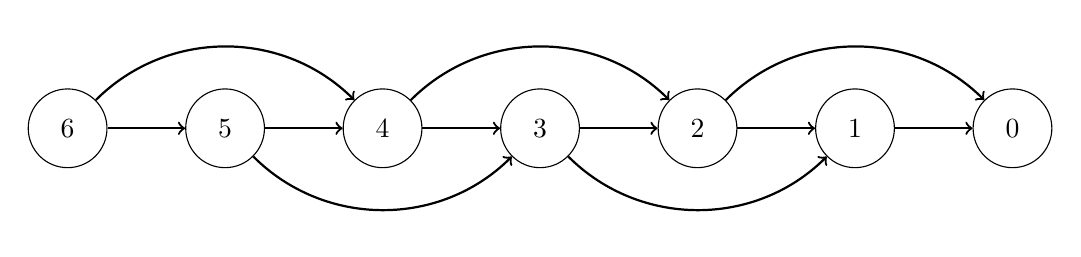
\begin{tikzpicture}[scale=1,place/.style={circle,draw, fill=white,inner sep=0pt,minimum size=10mm}]
    \node (P6)  at (0,0) [place] {6};
    \node (P5)  at (2,0) [place] {5};
    \node (P4)  at (4,0) [place] {4};
    \node (P3)  at (6,0) [place] {3};
    \node (P2)  at (8,0) [place] {2};
    \node (P1)  at (10,0) [place] {1};
    \node (P0)  at (12,0) [place] {0};
    \draw [->, thick] (P6) -- (P5);
    \draw [->, thick] (P5) -- (P4);
    \draw [->, thick] (P4) -- (P3);
    \draw [->, thick] (P3) -- (P2);
    \draw [->, thick] (P2) -- (P1);
    \draw [->, thick] (P1) -- (P0);
    \draw [->, thick] (P6) to [out=45] (P4);
    \draw [->, thick] (P4) to [out=45] (P2);
    \draw [->, thick] (P2) to [out=45] (P0);
    \draw [->, thick] (P5) to [out=315, in=225] (P3);
    \draw [->, thick] (P3) to [out=315, in=225] (P1);
    \end{tikzpicture}
    \caption{fib(6)的子问题图}
    \label{Fig:SubproblemgraphOfFib6}
\end{figure*}

\begin{example}
Fibonacci函数的子问题图

对于递归的Fibonacci函数,fib(n),问题实例是非负整数,所以F的子问题图的
顶点也是自然数。有向边是$\{i \rightarrow i-1 | i \geq 2\}\bigcup \{i \rightarrow i-2 |i \geq 2\}$。
尽管图是无限的,但是对于任意计算fib(n)对应的子图(例如,可以从顶点n
出发到达的部分)仅有n+1个顶点和2n条边。图\ref{Fig:SubproblemgraphOfFib6}展示
了这个例子。
\end{example}

如果算法A总是可终结的,则它的子问题图必然是无循环的。有向无环图(DAGs)在
7.4.6小节中学习过,我们将有一个用到前面学习内容的机会。通过查找一个顶层递归
调用(称为A(p))产生的活动帧树,显然树中的每一条路径就对应于一条A(p)的子问题图
中的一条边,这条边以顶点P为起点,以基本情况为结束点。基本情况节点没有出的边。
在这个抽象图中顶点就是问题实例。有向边代表执行A(p)的过程中进行的递归调用。
考虑
\begin{definition}
递归算法的动态规划版本

给定递归算法A,A的动态规划版本记为DP(A),是一个
\end{definition}


\section{矩阵的乘法顺序问题}
本节中我们将解决矩阵乘法的顺序问题,这是一个动态规划的经典例子。在下一节
中我们将学习一个起源与这个问题更本不相同的另一个问题,但是有一个非常类似
的解决方法。两者和在一起是一个动态规划的好的入门。

本节的目的不是展示如何解决矩阵乘法的顺序问题,而是展示如何一步一步的使用
规则来开发动态规划算法。我们希望这里的规则能帮助读者解决新的问题,能让
读者有一种思想(什么时候该使用动态程序的策略)。但是因为我们要解释
矩阵乘法顺序问题的解决方案,所以这个问题的“待遇”会比较好。

\subsection{矩阵乘法顺序问题}
假设我们想求在一串矩阵的连乘式子中,最好的乘法顺序。我们使用普通的矩阵乘法
算法(算法1.2),每一次我们乘上两个矩阵。一个$p \times q$的矩阵乘以$q\times r$
的矩阵,需要作pqr次元素的乘法。这里可以有很重要的两点。第一,矩阵的乘法有
结合率,即$A(BC)=(AB)C$。第二,结合顺序的不同,工作量会有 很大的差别。考虑
下面的例子。

\begin{example}
不同的矩阵乘法顺序

我们要乘的矩阵的大小如下:
\begin{displaymath}
A_1 \times   A_2   \times   A_3    \times  A_4
30\times 1  1\times 40   40\times 10    10\times 25
\end{displaymath}
下面的计算展示了不同的乘法顺序的不同计算量。

\begin{displaymath}
\begin{aligned}
&((A_1A_2)A_3)A_4  \qquad   30\times 1\times 40+30\times 40\times 10+30\times 10\times 25 = 20700\\
&A_1(A_2(A_3A_4))  \qquad   40\times 10\times 25+1\times 40\times 25+30\times 1\times 25 = 11750\\
&(A_1A_2)(A_3A_4)  \qquad   30\times 1\times 40+40\times 10\times 25+30\times 10\times 25 = 41200\\
&A_1((A_2A_3)A_4)  \qquad   1\times 40\times 10+1\times 10\times 25+30\times 1\times 25 = 1400
\end{aligned}
\end{displaymath}
\end{example}

对于一般的问题,假设我们给出矩阵$A_1, A_2, \cdots , A_n$,这里$A_i$的维数是
$d_{i-1}\times d_i (1\leq i \leq n)$。我们必须作多少次乘法,最小的消耗是多少?
我们的消耗是元素乘法的次数。(当然还有一些函数调用的开销。)现在我们将注意力
放在找到最小消耗上;之后我们使算法“回忆”起最小是怎么达到的。我们将$A_k$和$A_{k+1}$
之间的乘法表示为第k次乘法。

\subsection{贪婪的尝试}
任何一种n-1次乘法的序列都是合法的,算法需要决定那一个的消耗是最小的。贪婪的
算法看上去是可行的。首先选择消耗最小的那次乘法,在这次乘法之后求出 矩阵的
维数变化,继续选择最小消耗的乘法,重复之。例10.4 就有这种策略。然而,在某些
3个矩阵的序列时(仅有两次乘法),这种策略会失败。另一种贪婪的策略在练习10.6中。
典型的,动态程序算法比贪婪算法要更耗费时间,所以仅在无法找到贪婪策略来求
最优时才使用动态程序算法。

\subsection{动态规划的解决方案}
我们的下一个尝试是开发出一种递归算法。假设,在选择第一个乘法之后(序列中的
位置i),我们递归解决剩下的最优化问题。我们对每一个i都当作有效的第一个选择
尝试一次,最后选择有最小组合消耗的i。这叫做回溯算法,因为在尝试每一个完整的
选择序列之后,算法回溯到最近的选择点之前,在尝试另一种选择;当这一点的选择
都尝试过之后,算法回溯到更早的选择点再尝试新的选择,继续直到所有的选择都
尝试过了。我们在8皇后问题见过这种方法(参看图7.14)

假设维数$d_0, \cdots, d_n$在数组dim中。我们保持数组不变,仅通过一个整数序列
来标识子问题,整数序列表示剩下矩阵维数的索引。一开始索引序列是$0, \cdots, n$。
注意所有的序列的索引除了第一个和最后一个,都对应乘法运算符。

在第一个选择i之后,剩下问题的索引序列是$0, \cdots, i-1, i+1, \cdots, n$。
就是说,选择的第一个乘法是$A_i\times A_{i+1}$,其维数是$d_{i-1}$,$d_i$和
$d_{i+1}$。令$B=A_i \times A_{i+1}$;则B的维数是$d_{i-1}\times d_{i+1}$。剩下
的子问题是乘
\begin{displaymath}
A_1\times \cdots \times A_{i-1} \times B \times  A_{i+2} \times \cdots \times A_n
\end{displaymath}
假设索引序列本身存储在0开始的数组seq中,len是seq的长度。方法的概要是
\begin{figure}
\begin{lstlisting}[language={Java},keywordstyle=\color{blue!70}, commentstyle=\color{red!50!green!50!blue!50}]
mmTry1(dim, len, seq)
{
    if(len<3)
        bestCost=0;  //`基本情况一个数组或是没有`
    else
    {   bestCost=`$\infty$`;
        for(i=1; i<=len-1; i++)
        {
            c=seq[i]`的位置做乘法的消耗`;
            newSeq= seq`除去第i个元素`;
            b= mmTry1(dim, len-1, newSeq);
            bestCost=min(bestCost, b+c);
        }
    }
    return bestCost;
}
\end{lstlisting}
\end{figure}

这个算法的递归等式是$T(n)=(n-1)T(n-1)+n$ 。这个解决方案在$\Theta((n-1)!)$,
但是我们的目标是通过将递归算法转换成动态规划算法来提升性能。

为了设计一个动态规划的版本,我们首先需要分析子问题图。从初始的问题可以到达
多少子问题,就是索引序列$0, \cdots,n$可以描述多少问题?这里我们遭遇了一个
系列困难。尽管子序列是以更短的子区间开始的,但是随着子问题深度的不断加深,
他们会变成越来越多的片段。例如当n=10的时候,选择了子序列1,4,6,9,剩下的索引
变成了0,2,3,5, 7, 9,10。没有简单的方式来指定子序列。本质上来说,初时序列的
每一个子序列(至少带3个元素的)都是一个可到达的子问题。这里有$2^n$个这样的
子序列(参看练习10.3),因此有指数量级的子问题。这个图大到无法有效的查找了。

这个展示了设计动态规划算法最重要的法则。子问题必须有简单标识。这限制了
子问题图的最大规模(顶点的数量--还是可能有许多的边),并且可以为所有的
标识编制字典(在需要解决的范围内\footnote{译注:即给定问题规模其子问题的规模是
可以控制的})。回顾标识,或id的含义,一个元素的标识在字典中唯一的表示该
元素(2.5.3小节)。字典中不同的标识对应不同的元素。因此,只要我们将字典的大小
限制在输入的多项式时间之内,或者更小,那么我们就可以保证在深度优先搜索子问题图
时在多项式时间之内。

基于这些考虑,我们意识到我们需要不同的思路来将问题压缩成子问题。在第一个矩阵
乘法之后查找创建的子问题没有工作。通过选择最后一个矩阵乘法创建的子问题怎么样?
假设最后一个矩阵乘法的位置是i?这实际上创建了两个子问题:
\begin{enumerate}
\item 乘以$A_1, \cdots, A_i$其维数索引是$0, \cdots, i$:
        \begin{displaymath}
            A_1(d_0\times d_1) \times A_2(d_1\times d_2)\times \cdots  \times A_i(d_{i-1}\times d_i) =B_1(d_0\times d_i)
        \end{displaymath}
\item 乘以$A_{i+1}, \cdots, A_n$其维数索引是$i, \cdots, n$:
        \begin{displaymath}
            A_{i+1}(d_i\times d_{i+1}) \times A_{i+2}(d_{i+1}\times d_{i+2})\times \cdots \times A_n(d_{n-1}\times d_n) =B_2(d_i\times d_n)
        \end{displaymath}
\end{enumerate}

最后一步乘以$B_1B_2$的消耗是$(d_0, d_1, d_n)$。

并不能立即观察出这比我们一开始的方式好在那里。但是我们注意到每一个子问题都
可以标识成一个整数对(目前为止)(0,i)和(i,n)。就是说,第一个子问题的
索引序列是$(0, 1, \cdots, i)$,但是既然元素是连续的,所以仅需要列出终点。
(一个对(j-1,j)表示$A_j$是单独的,消耗是0)就像前面说的,维数数组
$d_0, \cdots, d_n$不用改变,可以作为一个全局的数组。

在进一步检查之前,我们看到一旦在子问题上选择了最后一个乘法的索引,创建出来
的新子问题也可以用一个整数对来描述。例如,如果在子问题(i,n)中选择了k,新的
子问题是(i,k)和(k,n)。因此我们看到这种问题分解方法仅在子问题图中创建了
$\Theta(n^2)$个不同子问题。

就像前面一样,我们不知道最后选择那一个乘法会有多少开销,所以我们需要枚举
所有的选择。mmTry2(dim,low, high)的目标就是找到(low,high)指定的子问题的
最优消耗,这里low<high。其概要类似与mmTry1:
\begin{figure}
\begin{lstlisting}[language={Java},keywordstyle=\color{blue!70}, commentstyle=\color{red!50!green!50!blue!50}]
    mmTry2(dim, low, high)
    {
    1.  if(high-low==1)
    2.      bestCost=0; // `基本情况:仅有一个矩阵`
    3.  else
    4.      bestCost=`$\infty$`;
    5.  for(k=low+1; k<=high-1; k++)
        {
    6.      a=mmTry2(dim, low, k);
    7.      b=mmTry2(dim, k, high);
    8.      c=`位置k处乘法的消耗`, dim[low], dim[k], dim[high]
    9.      bestCost=min(bestCost, a+b+c);
        }
    10. return bestCost;
    }
\end{lstlisting}
\end{figure}
与mmTry1类似,这也是一个回溯算法。这个算法的精确递归等式是复杂的,但是我们
可以得到一个简化的版本显示其大于$2^n$(参看练习10.4)。我们预计到这一点,
因为,回溯算法典型的都是指数级别的,但是我们希望可以通过把自然的递归算法
转换成动态规划来改进性能。

再一次的,让我们考虑子问题图,这里初始的问题用对(0,n)描述。顶点(子问题图的)
通过整数对(i,j)标识,i<j且i,j都在0,…,n的范围内,所以有约$n^2/2$个。对于对(i,j)
标识的子问题……

在下一个过程里,字典叫cost,其元素的标识是一对整数。为了使用通用ADT,我们
必须将标识包装进一个组织者类,但我们可以定制的字典的接口,使之接受两个整数,
low和high作为两个参数。我们依然使用字典的操作create, member, retrieve和store。
行号与mmTry2区别。
\begin{figure}
\begin{lstlisting}[language={Java},keywordstyle=\color{blue!70}, commentstyle=\color{red!50!green!50!blue!50}]
    mmTry2DP(dim, low, high, cost)
    {
    1.  if(high-low==1)
    2.      bestCost=0; // `基本情况:仅有一个矩阵`
    3.  else
    4.      bestCost=`$\infty$`;
    5.  for(k=low+1; k<=high-1; k++)
        {
    6a.     if(member(low, k)==false)
    6b.         a=mmTry2DP(dim, low, k, cost);
    6c.     else
    6d.         a=retrieve(cost,low, k);

    7a.     if(member(k, high)==false)
    7b.         b=mmTry2DP(dim, k, high, cost);
    7c.     else
    7d.         b=retrieve(cost, k, high);

    8       c=`位置k处乘法的消耗`, dim[low], dim[k], dim[high]
    9       bestCost=min(bestCost, a+b+c);
        }
    10a.    store(cost, low, high,bestCost);
    10b.    return bestCost;
    }
\end{lstlisting}
\end{figure}

既然子问题通过范围$0, \cdots, n$之内的整数对标识,那么字典可以用一个$(n+1)\times (n+1)$
矩阵来实现。在mmTry2DP中我们存储和检索子问题的最优解。在后面完整的算法里,
cost数组通过last数组来支持,last数组包含了子问题的最优选择乘法。无穷的条目
标识子问题还没有解决。我们将取消字典,直接访问数组。

我们已经看到mmTry2可以通过一些机械的步骤就转换成mmTry2DP,其实现了memo-ization。
结果看上去很像DFS的框架:第6和第7行在一个循环中测试没有解决的子问题(没有发现的,
或是白顶点),这个循环遍历了所有需要的问题(所有到邻接顶点的边)。已解决的子问题
(黑顶点)仅仅查找一下。在第10行(postorder time)当前子问题变成已解决了
(当前顶点标记为黑)。
。。。。。。。。。

从前一段提到的边,我们发现,减少第二个索引保持第一个索引将导致更低的拓扑数。


\section{构造最优二叉树}
在本节中我们考虑这样一个问题,如果我们知道对有些关键字的查找次数多于其他的,
怎样在二叉查找树中排列关键字(来源于线型集合)使得平均查找次数最小。 在
二叉查找树节点上的关键字符合定义6.3中给出的二叉查找树属性。回顾一下,以
中序遍历二叉查找树得到的是关键字的升序序列。看图10.3的例子。读者可能希望
在学习之前复习一下二叉查找树的遍历算法(算法6.1)。
\begin{definition}\vspace{1ex}
我们采用下面的记号:
\begin{enumerate}
\item 定义A(low, high, r)为子问题(low, high)是$K$被选为二叉查找树的根时的最小权消耗。
\item 定义A(low, high)是子问题(low, high)对于所有根的最小权消耗。
\item 定义$p(low,high)=p_{low}+\cdots+p_{high}$;就是说,概率that the key being
     search for is some key 在范围$K_{low}$到$K_{high}$中所有。我们称这个为
     \emph{子问题的权}(low, high)。
\end{enumerate}
\end{definition}
如果对于包含$K_{low}, \cdots, K_{high}$的特定树,其检索的消耗权是W(假定它是
一颗完整的树,所以它的根的深度是0),则如果它作为根的深度是1的子树时,则检索
的消耗权是(W+p(low, high))。就是说,每一次搜索穿过整个子树都比原来是完整树时
要多一次比较,所以多出的部分是p(low, high)。(参看插图10.4)这个关系允许我们
递归的合并子问题的解决方案得到更大问题的解决方案。

\begin{equation}
\begin{aligned}
A(low,high,r) &= p_r + p(low, r-1) +A(low, r-1)+ p(r+1, high)+A(r+1, high)
              &= p(low, high)+A(low,r-1)+A(r+1, high)
\end{aligned}
\end{equation}

\begin{equation}
A(low, high)= \min{A(low,highr, r)|low\leq r \leq high}
\end{equation}

我们可以写一个递归过程计算A(low, high),基于等式(10.2)和(10.3)。但是,就像
我们在10。3节学习的矩阵乘法顺序问题,我们将在递归解决方案观察到许多重复的工作。
算法运行时间将是指数时间。再一次,为了避免重复工作,我们定义一个字典,用大小
$(n+2)\times (n+1)$的两个二维数组,叫做cost和root。

就像在矩阵乘法顺序问题,子问题
